\documentclass[a4paper]{article}
\usepackage[14pt]{extsizes} % для того чтобы задать нестандартный 14-ый размер шрифта
\usepackage[utf8]{inputenc}
\usepackage[russian]{babel}
\usepackage{setspace,amsmath}
\usepackage[left=20mm, top=15mm, right=15mm, bottom=15mm, nohead, footskip=10mm]{geometry}
\usepackage{graphicx}
\usepackage{float}
\usepackage[usenames,dvipsnames]{color}
\usepackage{listings}
\DeclareGraphicsExtensions{.pdf,.png,.jpg}
\setlength{\parindent}{5ex}
\setlength{\parskip}{1em}
\lstset{ 
	language=Matlab,                		% choose the language of the code
%	basicstyle=10pt,       				% the size of the fonts that are used for the code
	numbers=left,                  			% where to put the line-numbers
	numberstyle=\footnotesize,      		% the size of the fonts that are used for the line-numbers
	stepnumber=1,                   			% the step between two line-numbers. If it's 1 each line will be numbered
	numbersep=5pt,                  		% how far the line-numbers are from the code
%	backgroundcolor=\color{white},  	% choose the background color. You must add \usepackage{color}
	showspaces=false,               		% show spaces adding particular underscores
	showstringspaces=false,         		% underline spaces within strings
	showtabs=false,                 			% show tabs within strings adding particular underscores
%	frame=single,	                			% adds a frame around the code
%	tabsize=2,                				% sets default tabsize to 2 spaces
%	captionpos=b,                   			% sets the caption-position to bottom
	breaklines=true,                			% sets automatic line breaking
	breakatwhitespace=false,        		% sets if automatic breaks should only happen at whitespace
	escapeinside={\%*}{*)}          		% if you want to add a comment within your code
}
% настройки полей документа
 
\begin{document} % начало документа
 
% НАЧАЛО ТИТУЛЬНОГО ЛИСТА
\begin{center}
\hfill \break
\normalsize{Министерство Образования и науки Российской Федерации}\\
\hfill \break
\normalsize{Федеральное государственное автономное образовательное учреждение высшего образования}\\ 
\hfill \break
\normalsize{САНКТ-ПЕТЕРБУРГСКИЙ НАЦИОНАЛЬНЫЙ ИССЛЕДОВАТЕЛЬСКИЙ}\\
\normalsize{«УНИВЕРСИТЕТ ИТМО»}\\
\hfill \break
\hfill \break
\hfill \break
\hfill \break
 \hfill \break
\normalsize{Кафедра систем управления и робототехники}\\
\hfill\break
\hfill \break
\hfill \break
\hfill \break
\normalsize{Отчет по лабораторной работе №7}\\
\normalsize{"Разработка системы управления для неполноприводного робота"\ }\\
\hfill \break
\hfill \break
\hfill \break
\hfill \break
\hfill \break
\begin{flushright}
   \begin{tabular}{r r}
   Выполнил: &  студент группы R3136\\
  & Шахтаров Иван\\
  Преподаватель: & Перегудин А.А\\
  \end{tabular}
\end{flushright}
 \hfill \break
\hfill \break
\hfill \break
\hfill \break
\hfill \break
\hfill \break
\hfill \break
\hfill \break
\hfill \break
\hfill \break
\end{center}
\begin{center} Санкт-Петербург 2020\end{center}
\thispagestyle{empty} % выключаем отображение номера для этой страницы
 
% КОНЕЦ ТИТУЛЬНОГО ЛИСТА

% Введение
\newpage
\section{Цель работы}
\begin{flushleft}
Получить опыт составления модели вход-состояние-выход для относительно сложного электромеханического устройства. Познакомиться с понятием П-регулятора состояния, расчетом его коэффициентов и принципами работы неполноприводных роботов, находящихся под его управлением.    
\end{flushleft}

\section{Расчет характеристик робота}
\begin{flushleft}
Для составления успешной математической модели необходимы следующие данные о роботе:
\end{flushleft}

\begin{enumerate}
    \item \(k_m, k_e\) - конструктивные постоянные двигателя
    \item \(m_{\text{т}}, m_{\text{к}}\) - масса тележки\footnote{Сюда входит брик, два двигателя и датчик} и колеса\footnote{Шина + колесо} соответственно
    \item \(L\) - длина тележки
    \item \(R\) - сопротивление двигателя
    \item \(r\) - радиус колеса
    \item \(J, J_{\text{т}}, J_{\text{к}}\) - моменты инерции(отн. собственных центров масс) для двигателя, тележки и колеса соответственно
\end{enumerate}

\begin{flushleft}
Из прошлых лабораторных работ мы знаем, что:
    \begin{equation*}
        k_m = k_e = 0.29
    \end{equation*}
    \begin{equation*}
        R = 4.7 \text{ Ом}
    \end{equation*}
    \begin{equation*}
        J = 0.0023 \text{ кг} \cdot \text{м}^2
    \end{equation*}
\end{flushleft}

\begin{flushleft}
Из-за отсутствия возможности измерить \(m_{\text{т}}, m_{\text{к}}, L\), эти данные были найдены в интернете:
    \begin{equation*}
        L = 0.111 \text{ м}
    \end{equation*}
    \begin{equation*}
        m_{\text{т}} = 0.330 \text{ кг}
        \footnote{Источник: http://home.agh.edu.pl/~ap/segway/docs/nxt-lego-part-weights.pdf}
    \end{equation*}
    \begin{equation*}
        m_{\text{к}} = 0.018 \text{ кг} \footnote{Источник: http://wheels.sariel.pl/}
    \end{equation*} 
    \begin{equation*}
        r = 0.028 \text{ м}^4
    \end{equation*}
\end{flushleft}
\hfill \break
\begin{flushleft}
Моменты инерции для двигателя и тележки вычислим по известным из курса физики формулам, представив тележку, как набор кубоидов, а колесо, как цилиндр:
\begin{equation*}
    J_{\text{к}} = \frac{mr^2}{2} = \frac{0.018 \cdot 0.028^2}{2} = 0.007056 \text{ г} \cdot \text{м}^2
\end{equation*}

Для вычисления \(J_{\text{т}}\)\ воспользуемся свойством аддитивности момента инерции и теоремой Штейнера. Для лучшего понимания снизу представлены приблизительные чертежи робота (все измерения в мм):

\begin{figure} [!ht]
    \center{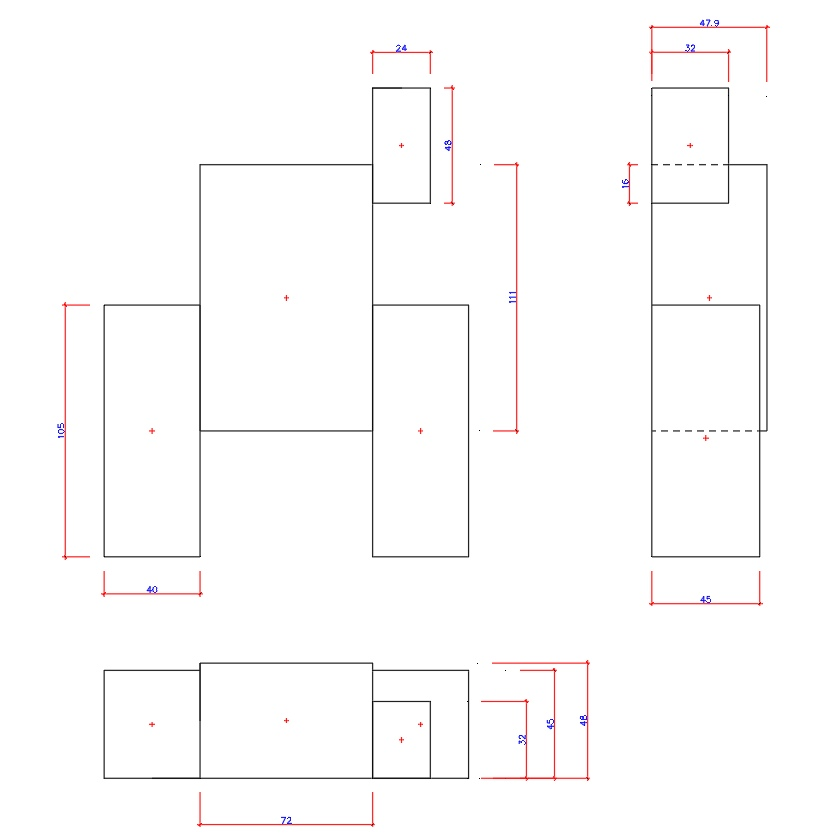
\includegraphics[width=450pt]{4.jpg}}
    \caption{Чертеж робота}
\end{figure}

\begin{figure} [!ht]
    \center{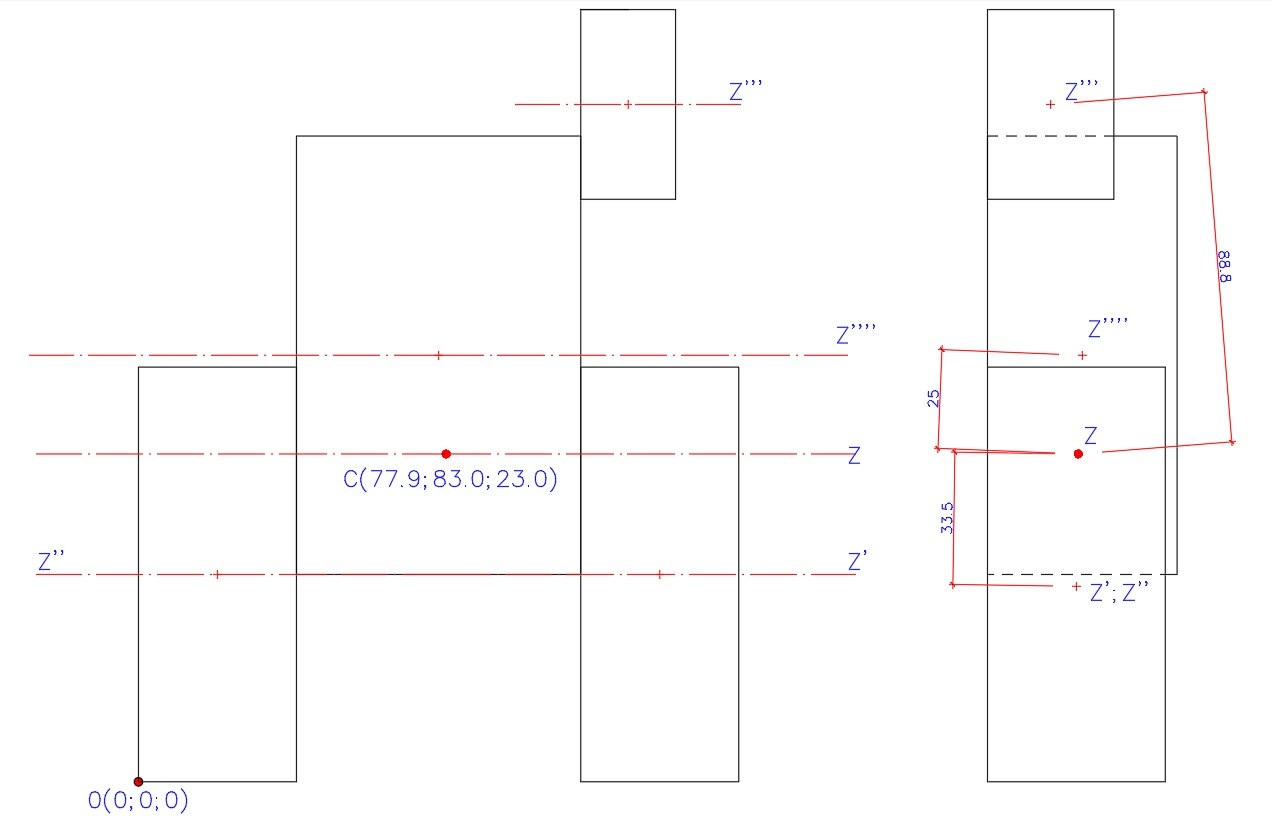
\includegraphics[width=450pt]{5.jpg}}
    \caption{Расположение осей симметрии}
\end{figure}

\hfill \break
\hfill \break
При помощи легко гуглящихся формул найдем координаты центра масс нашего робота. Для этого будем считать, что центр масс каждого кубоида совпадает с его геометрическим центром:
\begin{equation*}
    \vec{r}_c = \frac{\sum m_i \vec{r}_i}{\sum m_i}
\end{equation*}
где \(m_{i}, \vec{r}_{i}\)\ - масса и радиус вектор центра масс i-того кубоида
\begin{equation*}
    \vec{r}_c = \frac{0.08\begin{pmatrix} 20\\52.5\\22.5 \end{pmatrix} + 0.08\begin{pmatrix} 134\\52.5\\22.5 \end{pmatrix} + 0.16\begin{pmatrix} 76\\108\\24 \end{pmatrix} + 0.01\begin{pmatrix} 124\\171.5\\16\\ \end{pmatrix}}{0.08+0.08+0.16+0.01} = \begin{pmatrix} 77.9\\83.0\\23.0 \end{pmatrix}
\end{equation*}
Теперь, зная координаты центра масс системы, можно расположить ось симметрии Z и уже относительно нее рассчитать момент инерции \(J_{\text{т}}\)\ с помощью следующей формулы:
\begin{equation}
    J_{\text{т}} = J_{\text{брик}} + 2J_{\text{дпт отн. Z}} + J_{\text{датчик отн. Z}} 
\end{equation}
Оси \(Z'\)\ и \(Z''\)\ совпадают, тогда пусть \(ZZ' = ZZ'' = 0.0335 \text{ (м)} =b\)\
\newline
Также введем обозначение для \(ZZ''' = 0.0888 \text{ (м)} = c \)\ и  \(ZZ'''' = 0.025 \text{ (м)}  =a \)\

\begin{equation}
    J_{\text{брик}} = \frac{m_{\text{брик}}(h_{\text{брик}}^2+ d_{\text{брик}}^2)}{12} + m_{\text{брик}}a^2= 0.000295 \text{ кг} \cdot \text{м}^2
\end{equation}
\begin{equation}
    J_{\text{дпт}} = \frac{m_{\text{дпт}}(h_{\text{дпт}}^2+ d_{\text{дпт}}^2)}{12} + m_{\text{дпт}} b^2 = 0.000177 \text{ кг} \cdot \text{м}^2
\end{equation}
\begin{equation}
    J_{\text{датчик}} = \frac{m_{\text{датчик}}(h_{\text{датчик}}^2+ d_{\text{датчик}}^2)}{12} + m_{\text{датчик}} c^2 = 0.0000816 \text{ кг} \cdot \text{м}^2
\end{equation}
где \(h_{i}, d_{i}\)\ - высота и длина нужного кубоида соответственно
\newline
Подставив полученные в (2)-(4) значения в (1) получаем, что
\begin{equation*}
    J_{\text{т}} = 0.00073 \text{ кг} \cdot \text{м}^2
\end{equation*}
\section{Расчет коэффициентов регулирования}
Используя вычисленные нами ранее параметры системы, составим матрицу управляемости \(Y_{3 \times 3}\)\ которая в нашем случае будет выглядеть, как \([B\text{ }AB\text{ }A^{2}B],\)\ где \(A_{3 \times 3}\)\ - матрица, определяющая динамические свойства объекта управления, а \(B_{3 \times 1}\)\ - матрица входа управляющих воздействий.
\begin{gather*}
A = 
    \begin{bmatrix}
    0 & 0 & 1\\
    \(\frac{m_{\text{т}}^{2}l^{2}gr}{\chi_1}\)\ & \(\frac{2k_{m}k_{e}( m_{\text{т}}lr + m_{\text{т}}l^2 + J_{\text{т}} )}{R\chi_1}\)\ & 0\\
    \(-\frac{m_{\text{т}}gl(m_{\text{т}}r^2 + 2m_{\text{к}}r^2 + 2J_{\text{к}} + 2J)}{\chi_1}\)\ & \(-\frac{2k_{m}k_{e}( m_{\text{т}}lr + m_{\text{т}}r^2 + 2m_{\text{к}}r^2 + 2J_{\text{к}} )}{R\chi_1}\)\ & 0\\
    \end{bmatrix}
\end{gather*}

\begin{gather*}
    B = 
    \begin{bmatrix}
    0\\
    \(-\frac{2k_{m}( m_{\text{т}}lr + m_{\text{т}}l^2 + J_{\text{т}} )}{R\chi_1}\)\\\
    \(\frac{2k_{m}( m_{\text{т}}lr + m_{\text{т}}r^2 + 2m_{\text{к}}r^2 + 2J_{\text{к}} )}{R\chi_1}\)\\\
    \end{bmatrix}
\end{gather*}
где \(\chi_1 = m_{\text{т}}lr(m_{\text{т}}lr-2J)-(m_{\text{т}}l^2+J_{\text{т}})(m_{\text{т}}r^2+2m_{\text{к}}r^2 + 2J_{\text{к}}+ 2J),\)\ а \(l=\frac{L}{2}\)\
\newline
Подставив числовые значения, получим следующее:
\begin{equation*}
    \chi_1 = -1.07 \cdot 10^{-5}
\end{equation*}
\begin{gather*}
A=
    \begin{bmatrix}
    0 & 0 & 1\\
    -8.6381 & -7.5880 & 0\\
    82.5553 &  2.7334 & 0\\
    \end{bmatrix}
, B=
    \begin{bmatrix}
    0 \\
    26.1654 \\
    -9.4256 \\
    \end{bmatrix}
\end{gather*}
\begin{gather*}
Y=
    \begin{bmatrix}
    0 & -0.0094 & 0.0715\\
    0.0262  &  -0.1985  &  1.5879  \\
   -0.0094  &  0.0715 &  -1.3208 \\
    \end{bmatrix}
\end{gather*}
\begin{equation*}
    det(Y) = -1.85 \cdot 10^{5} \neq 0
\end{equation*}
Из этого следует, что робот управляем
\newpage
Так как порядок объекта управления \(n\)\ в нашем случае равен 3, то стандартное время переходного процесса \(t_{\text{п}}^{*} = 6.3 \text{ с,}\)\ действительное же время переходного процесса возьмем равным \(t_{\text{п}} = 0.5 \text{ с,}\)\ тогда
\begin{equation*}
    \omega_0 = \frac{t_{\text{п}}^{*}}{t_{\text{п}}} = 12.6
\end{equation*}
Уравнение для вычисления матрицы коэффициентов \(K\)\ имеет вид:
\begin{equation*}
    \begin{bmatrix}
    k_1\\
    k_2\\
    k_3\\
    \end{bmatrix}
    =
    \begin{bmatrix}
    0 & b_2 & b_3\\
    b_3 & 0 & a_{32}b_{2} - a_{22}b_{3}\\
     a_{32}b_{2} - a_{22}b_{3} &  a_{21}b_{3} - a_{31}b_{2} & 0\\
    \end{bmatrix}^{-1}
    \begin{bmatrix}
    3\omega_0 + a_{22}\\
    3\omega_0^2 + a_{31}\\
    \omega_0^3 - a_{22}a_{31} + a_{21}a_{32}
    \end{bmatrix}
\end{equation*}
Подставив численные значения получаем:
\begin{equation*}
K=
    \begin{bmatrix}
    -59.2889 \\
   -1.2523 \\
   -6.6818 \\
    \end{bmatrix}
\end{equation*}
\section{Моделирование системы в Simulink}
Результат моделирования представлен на рисунках 3 и 4 ниже

\begin{figure} [H]
    \center{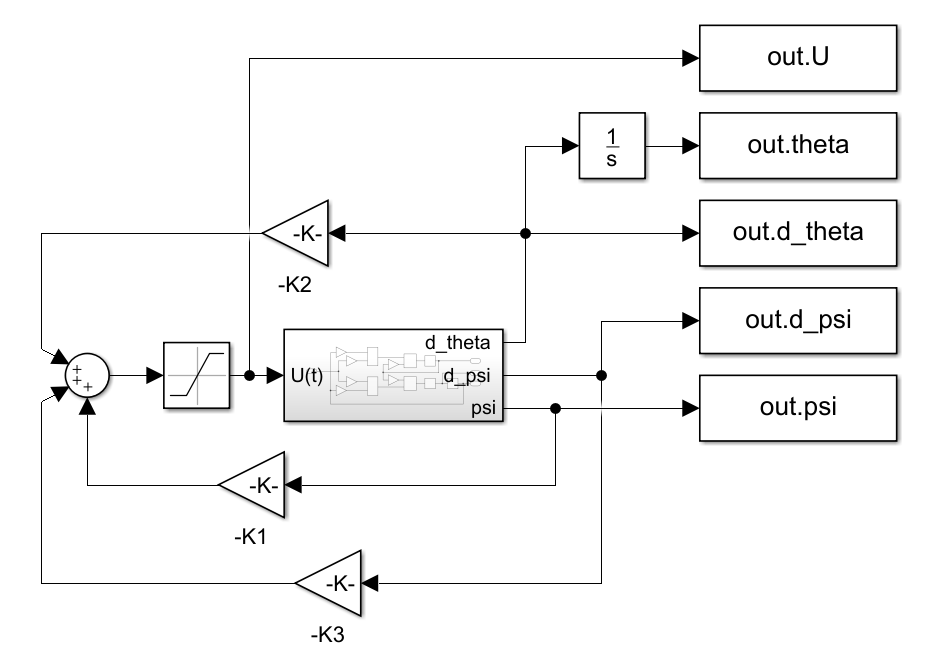
\includegraphics[width=470pt]{System.png}}
    \caption{Система}
\end{figure}

\begin{figure}[H]
    \center{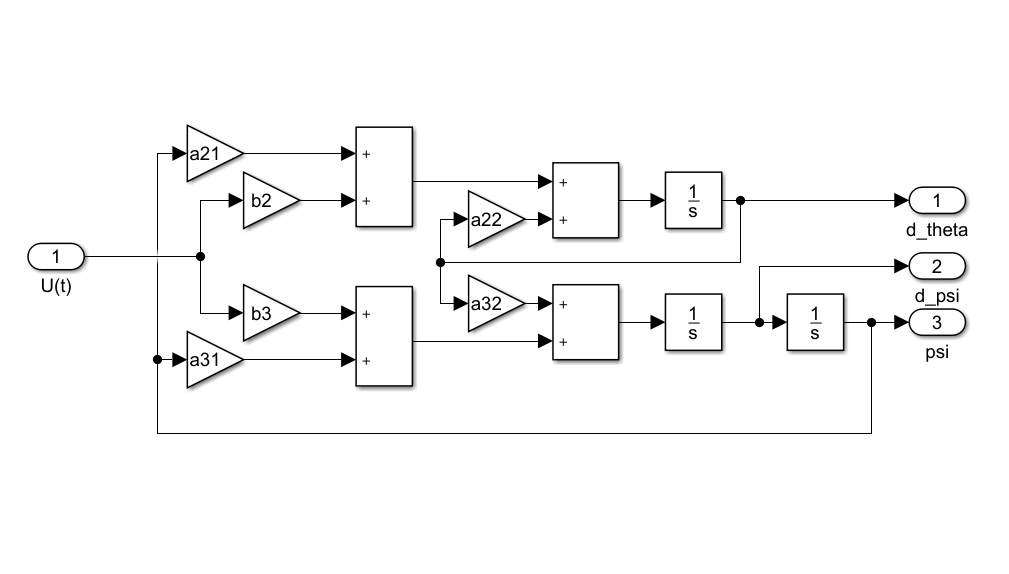
\includegraphics[width=470pt]{Subsystem.png}}
    \caption{Подсистема}
\end{figure}

Код в Matlab:
\lstinputlisting[language=Matlab]{main.m}


\section{Графики }
\begin{figure} [H]
    \center{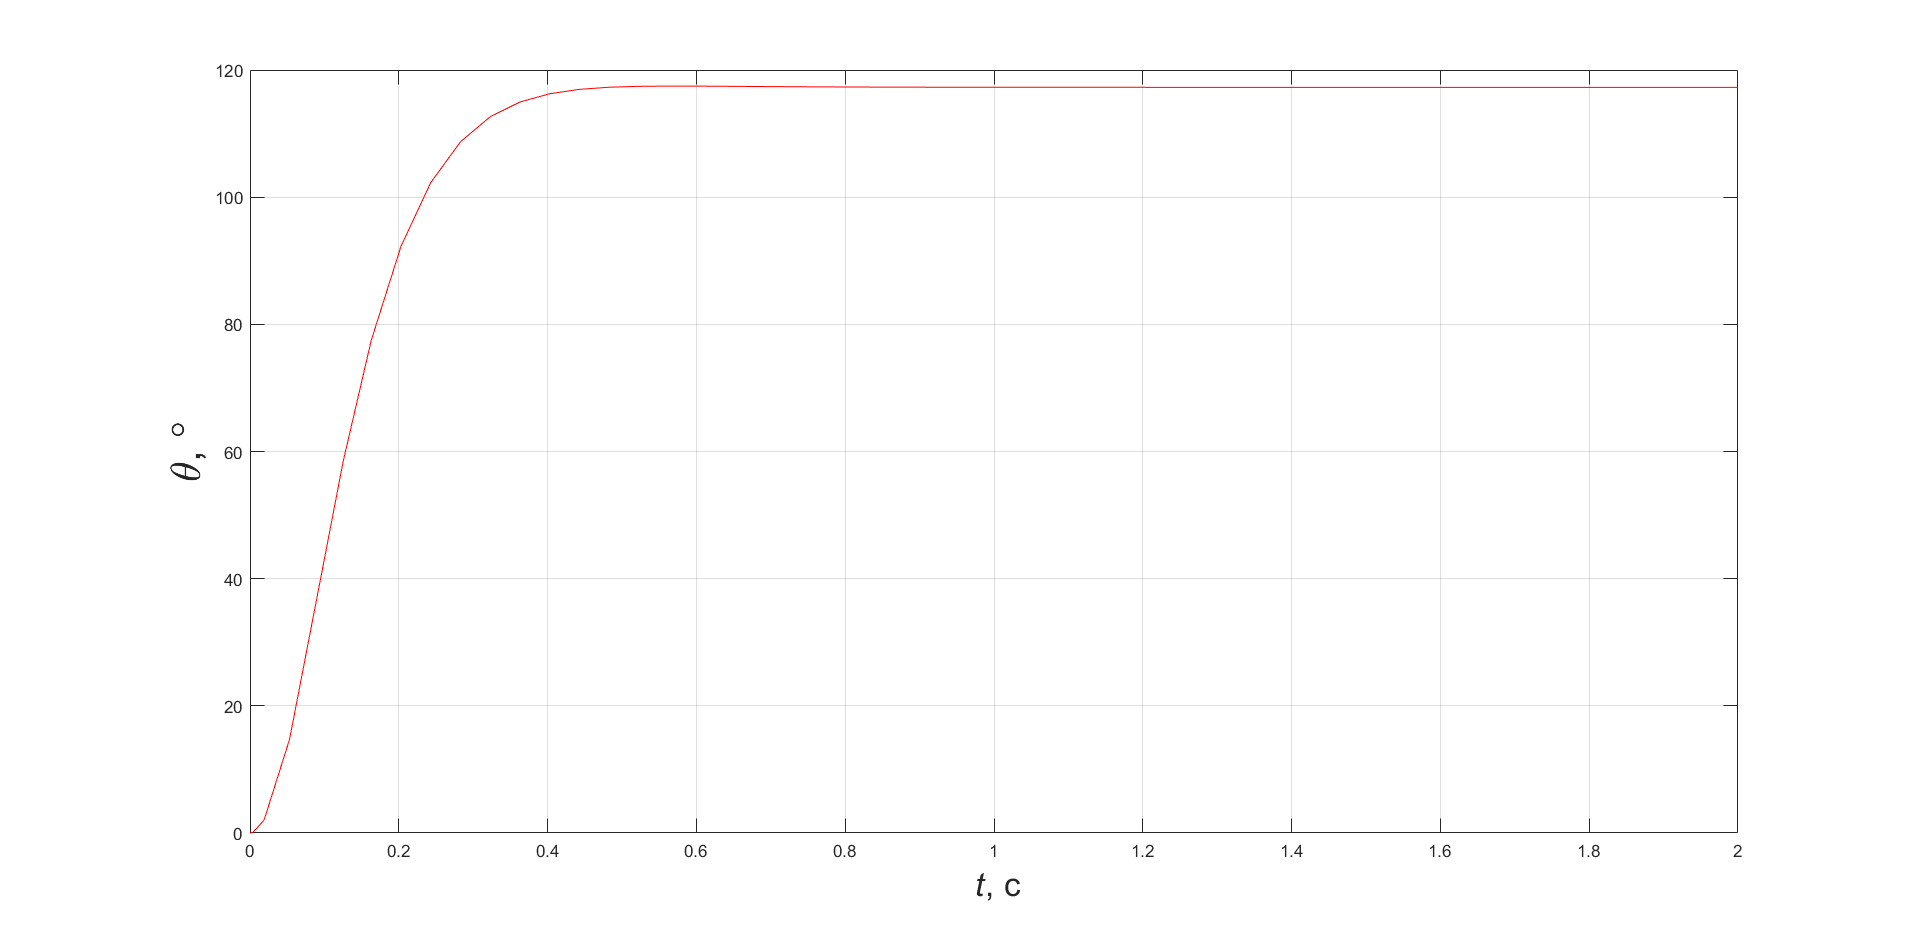
\includegraphics[width=500pt]{theta.png}}
    \caption{Зависимость \(\theta = \theta(t)\)\ }
\end{figure}

\begin{figure} [H]
    \center{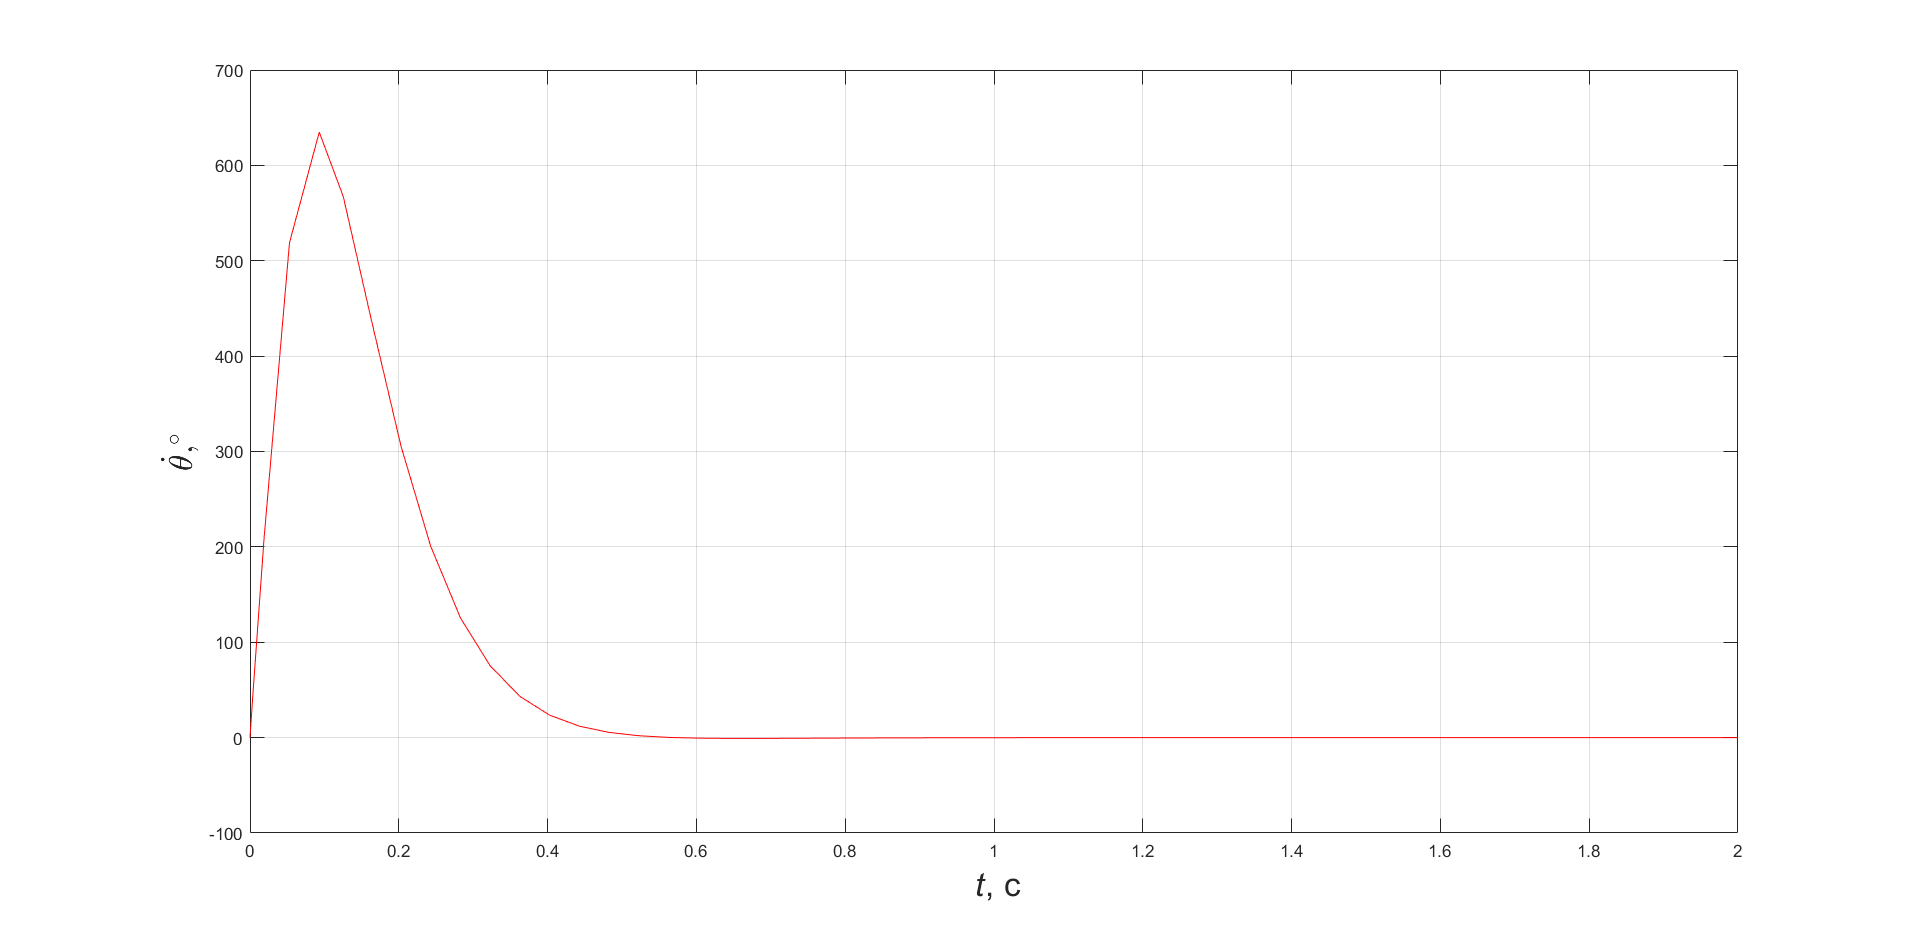
\includegraphics[width=500pt]{d_theta.png}}
    \caption{Зависимость \(\dot{\theta} = \dot{\theta}(t)\)\ }
\end{figure}

\begin{figure} [H]
    \center{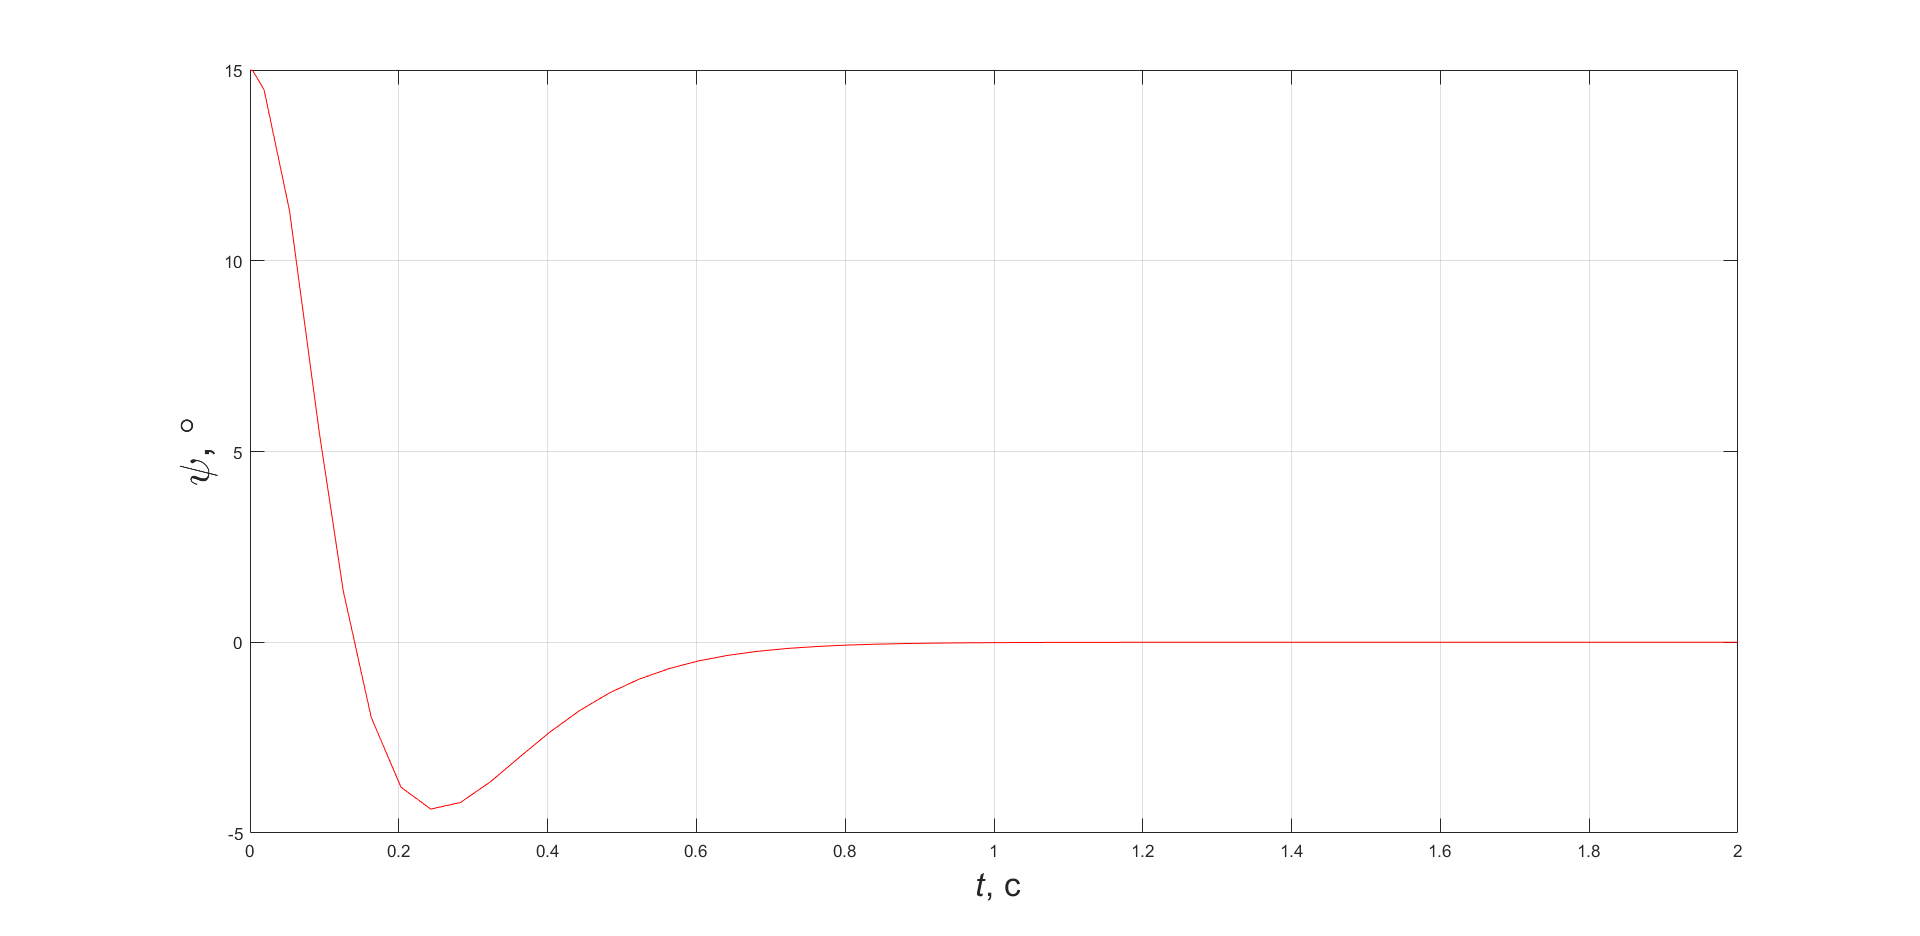
\includegraphics[width=500pt]{psi.png}}
    \caption{Зависимость \(\psi = \psi(t)\)\ }
\end{figure}

\begin{figure} [H]
    \center{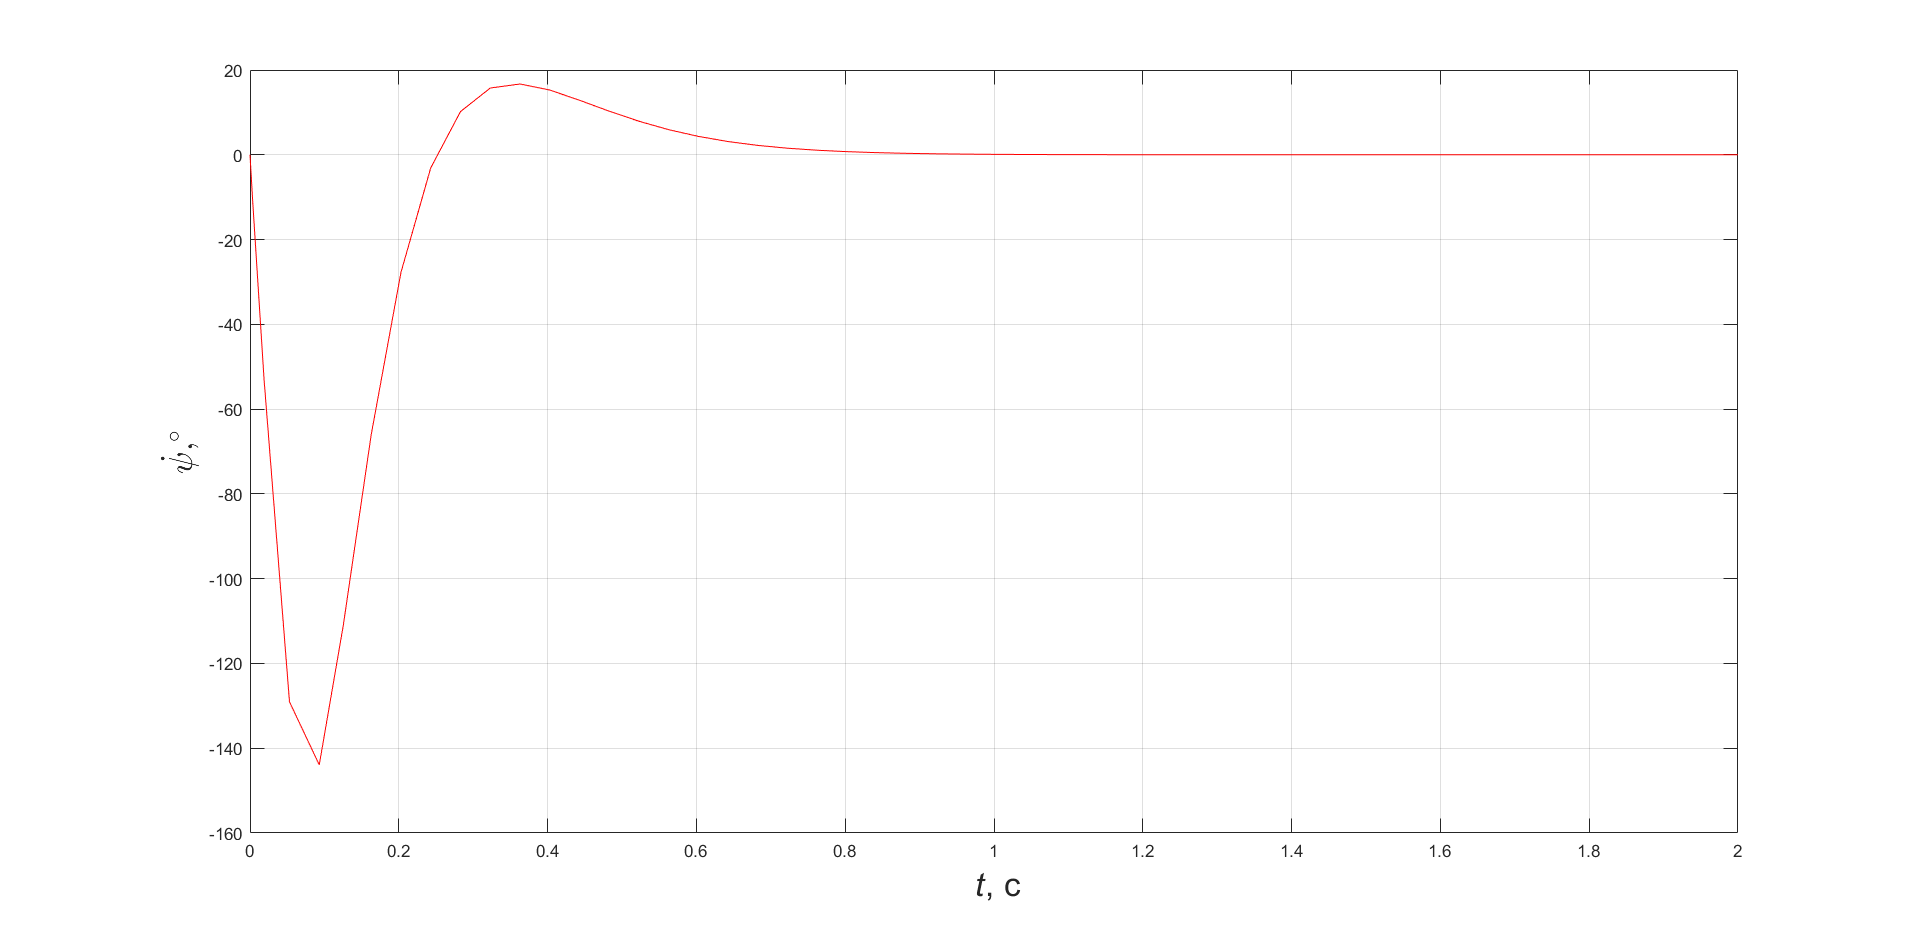
\includegraphics[width=500pt]{d_psi.png}}
    \caption{Зависимость \(\dot{\psi} = \dot{\psi}(t)\)\ }
\end{figure}

\begin{figure} [H]
    \center{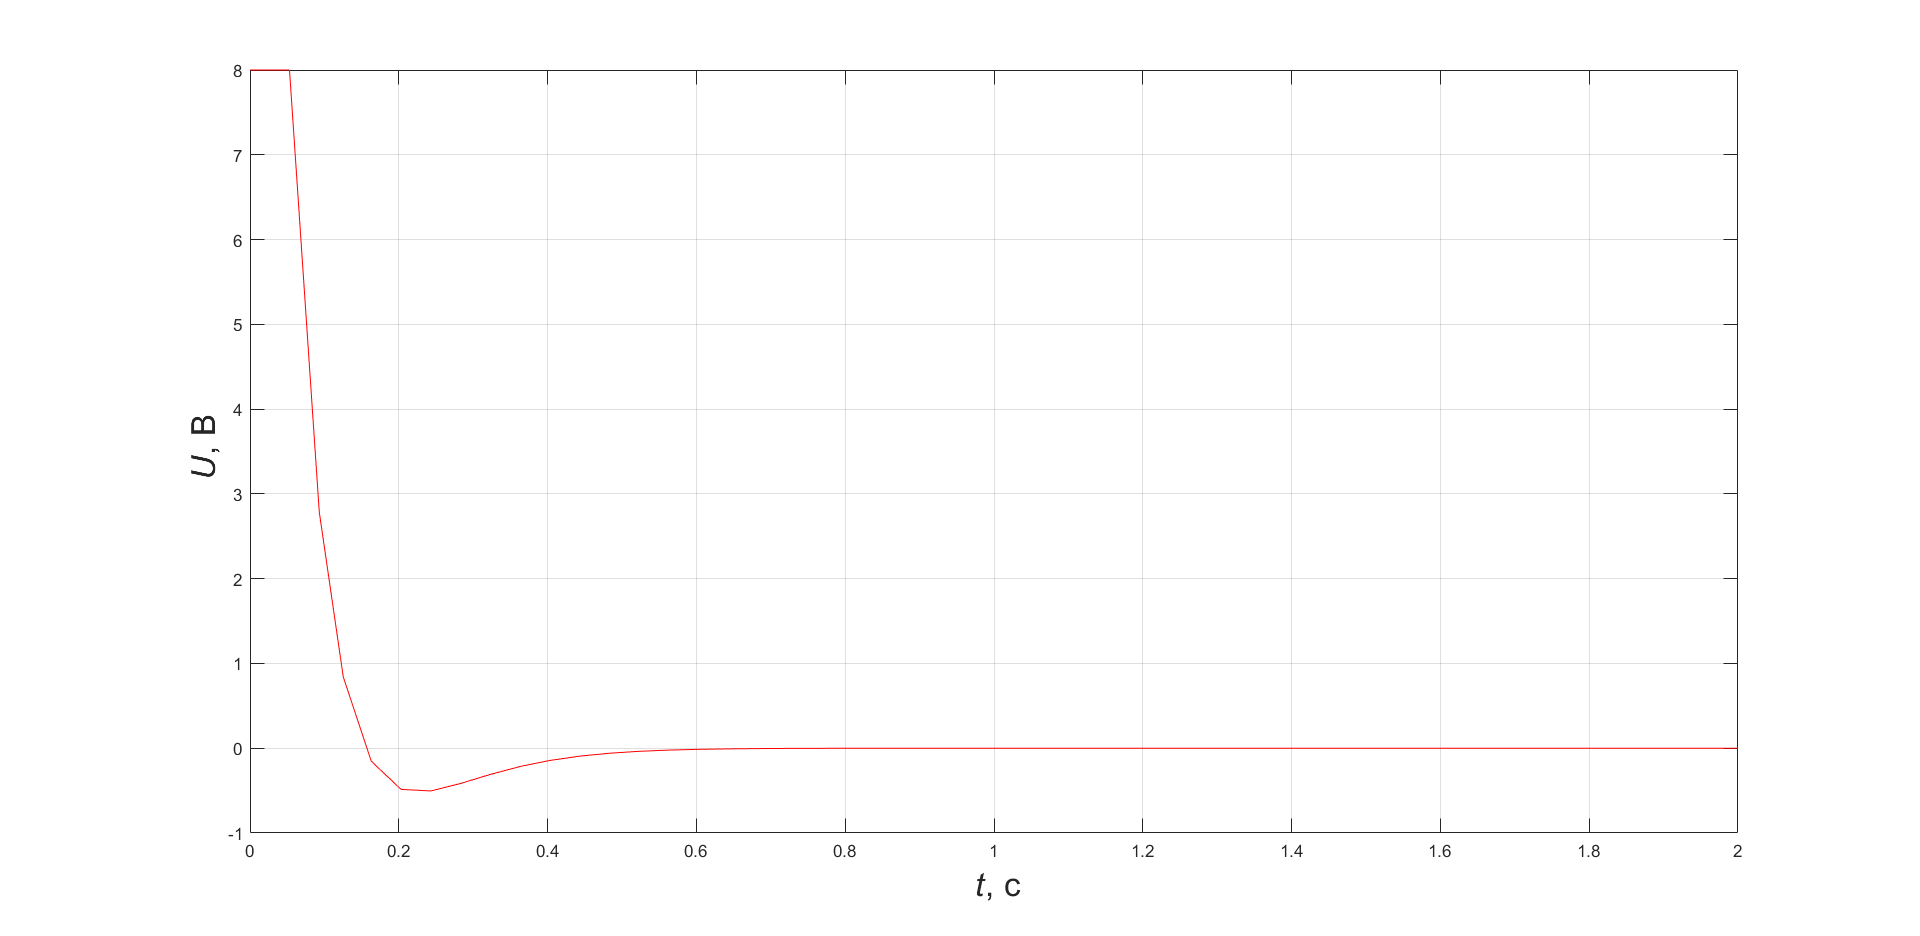
\includegraphics[width=500pt]{voltage.png}}
    \caption{Зависимость \(U = U(t)\)\ }
\end{figure}


\section{Вывод}
В ходе этой работы я получил опыт составления модели вход - состояние - выход, ознакомился с понятием П-регулятора состояния и научился работать в системе \LaTeX.
\end{flushleft} 
\end{document}
